

\input{../Latex_Templates/Preamble_Report}

%%%%% TITLE PAGE

%\subject{, VT23}
\title{ Report for the Course Modelling in Computational Science, HT23 \\[1ex]
	  \large Project 1: The Potts model}
%\subtitle{}
\author{Theo Koppenhöfer}
\date{Lund \\[1ex] \today}

\addbibresource{bibliography.bib}

\usepackage{pythonhighlight}
\graphicspath{{../Figures/}}

%%%%% The content starts here %%%%%%%%%%%%%


\begin{document}

\maketitle

\section{Introduction}

The following report is part of the first project of the Modelling in Computational Science course at Lund University, HT2023.
In the first project we implemented a Monte-Carlo simulation of the $q$-state Potts model.
The report and the Python implementation can be found online under \cite{Repository}

\section{The Potts model}

A state of the $q$-state Potts model of a $L\times L$ flat grid is given by a mapping
\begin{align*}
	s\colon \brk[c]{1,\dots,L}\times\brk[c]{1,\dots,L}\to\brk[c]{1,\dots,L}\,.
\end{align*}
One assigns this state an energy via
\begin{align*}
	E = -J\sum_{\substack{i, j\text{ neighbouring}\\ \text{grid points}}}\delta\brk*{s_i,s_j}
\end{align*}
where $\delta$ denotes the Kronecker-delta and $J=1$ is the coupling strength. As given in the problem setting we assume periodic boundary conditions on the grid.

\section{The implementation}

\subsubsection{Determining when the Energy has plateaued}

The energy of the system takes some time $t_0$ to reach an equilibrium state. To determine $t_0$ we calculate in every step $i$ moving averages $\text{ma}_1$ and $\text{ma}_2$ over $n$ energies. The construction is shown in figure \ref{fi:movingAverages}. If we start in the hot state then the energy will tend to shrink until we reach an equilibrium. Hence we can use the condition
\begin{align}
	\text{ma}_2 \leq \text{ma}_1 \label{eq:equilCondition}
\end{align}
to determine $t_0$. If on the other hand we start in cold state the energy will in general increase and we have to reverse the inequality in equation \eqref{eq:equilCondition}. After reaching an equilibrium the simulation runs for a further \pyth{M_sampling=5000} steps. It is over these samples we take the mean and the variance.

\begin{figure}
\centering
\input{../Figures/explanationMovingAverages.pdf_tex}
\caption{Explanation of the moving averages.}
\label{fi:movingAverages}
\end{figure}

\subsubsection{Improving performance}
While simulating we run into performance issues due to the fact that Python is in general rather slow even with heavy use of Numpy. We resolved this issue with the help of Numba which precompiled functions and thus increased performance substantially. The downside is that the code becomes quite unestetic because Numba only supports some Python and Numpy features.


\begin{figure}
\centering
% This file was created with tikzplotlib v0.10.1.
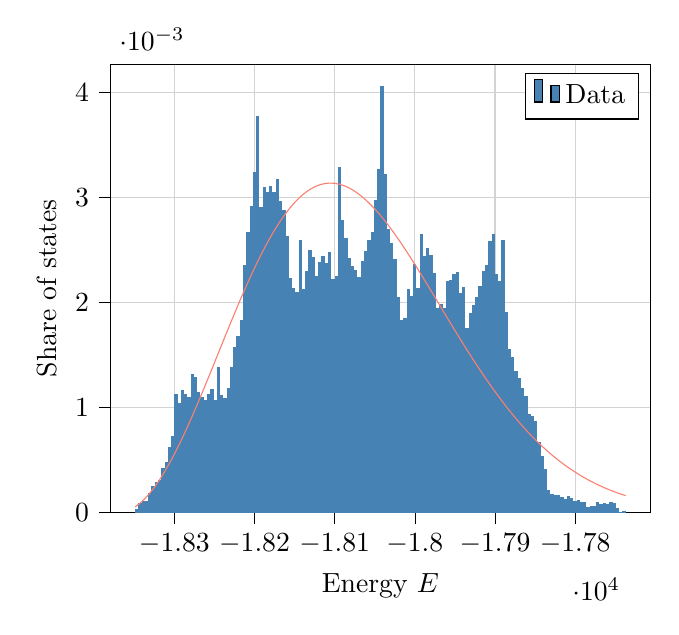
\begin{tikzpicture}

\definecolor{lightgray}{RGB}{211,211,211}
\definecolor{salmon}{RGB}{250,128,114}
\definecolor{steelblue}{RGB}{70,130,180}

\begin{axis}[
tick align=outside,
tick pos=left,
x grid style={lightgray},
xlabel={Energy \(\displaystyle E\)},
xmajorgrids,
xmin=-18379.6, xmax=-17706.4,
xtick style={color=black},
y grid style={lightgray},
ylabel={Share of states},
ymajorgrids,
ymin=0, ymax=0.00426613970588053,
ytick style={color=black}
]
\draw[draw=none,fill=steelblue] (axis cs:-18349,0) rectangle (axis cs:-18344.92,3.72549019607684e-05);
\addlegendimage{ybar,ybar legend,draw=none,fill=steelblue}
\addlegendentry{Data}

\draw[draw=none,fill=steelblue] (axis cs:-18344.92,0) rectangle (axis cs:-18340.84,9.28921568627882e-05);
\draw[draw=none,fill=steelblue] (axis cs:-18340.84,0) rectangle (axis cs:-18336.76,0.000113235294117599);
\draw[draw=none,fill=steelblue] (axis cs:-18336.76,0) rectangle (axis cs:-18332.68,0.000109803921568678);
\draw[draw=none,fill=steelblue] (axis cs:-18332.68,0) rectangle (axis cs:-18328.6,0.000182843137254824);
\draw[draw=none,fill=steelblue] (axis cs:-18328.6,0) rectangle (axis cs:-18324.52,0.0002497549019609);
\draw[draw=none,fill=steelblue] (axis cs:-18324.52,0) rectangle (axis cs:-18320.44,0.000285784313725368);
\draw[draw=none,fill=steelblue] (axis cs:-18320.44,0) rectangle (axis cs:-18316.36,0.000308333333333476);
\draw[draw=none,fill=steelblue] (axis cs:-18316.36,0) rectangle (axis cs:-18312.28,0.000426225490195896);
\draw[draw=none,fill=steelblue] (axis cs:-18312.28,0) rectangle (axis cs:-18308.2,0.000482352941176694);
\draw[draw=none,fill=steelblue] (axis cs:-18308.2,0) rectangle (axis cs:-18304.12,0.000626470588235026);
\draw[draw=none,fill=steelblue] (axis cs:-18304.12,0) rectangle (axis cs:-18300.04,0.000726715686274847);
\draw[draw=none,fill=steelblue] (axis cs:-18300.04,0) rectangle (axis cs:-18295.96,0.00112499999999952);
\draw[draw=none,fill=steelblue] (axis cs:-18295.96,0) rectangle (axis cs:-18291.88,0.00104215686274558);
\draw[draw=none,fill=steelblue] (axis cs:-18291.88,0) rectangle (axis cs:-18287.8,0.00116764705882303);
\draw[draw=none,fill=steelblue] (axis cs:-18287.8,0) rectangle (axis cs:-18283.72,0.00113210784313778);
\draw[draw=none,fill=steelblue] (axis cs:-18283.72,0) rectangle (axis cs:-18279.64,0.0010963235294113);
\draw[draw=none,fill=steelblue] (axis cs:-18279.64,0) rectangle (axis cs:-18275.56,0.00132058823529473);
\draw[draw=none,fill=steelblue] (axis cs:-18275.56,0) rectangle (axis cs:-18271.48,0.00128700980392102);
\draw[draw=none,fill=steelblue] (axis cs:-18271.48,0) rectangle (axis cs:-18267.4,0.00114901960784367);
\draw[draw=none,fill=steelblue] (axis cs:-18267.4,0) rectangle (axis cs:-18263.32,0.00110171568627404);
\draw[draw=none,fill=steelblue] (axis cs:-18263.32,0) rectangle (axis cs:-18259.24,0.00106764705882402);
\draw[draw=none,fill=steelblue] (axis cs:-18259.24,0) rectangle (axis cs:-18255.16,0.00112549019607795);
\draw[draw=none,fill=steelblue] (axis cs:-18255.16,0) rectangle (axis cs:-18251.08,0.00117254901960839);
\draw[draw=none,fill=steelblue] (axis cs:-18251.08,0) rectangle (axis cs:-18247,0.00107205882352895);
\draw[draw=none,fill=steelblue] (axis cs:-18247,0) rectangle (axis cs:-18242.92,0.00138946078431313);
\draw[draw=none,fill=steelblue] (axis cs:-18242.92,0) rectangle (axis cs:-18238.84,0.00111495098039267);
\draw[draw=none,fill=steelblue] (axis cs:-18238.84,0) rectangle (axis cs:-18234.76,0.00109191176470541);
\draw[draw=none,fill=steelblue] (axis cs:-18234.76,0) rectangle (axis cs:-18230.68,0.0011867647058829);
\draw[draw=none,fill=steelblue] (axis cs:-18230.68,0) rectangle (axis cs:-18226.6,0.00138382352941117);
\draw[draw=none,fill=steelblue] (axis cs:-18226.6,0) rectangle (axis cs:-18222.52,0.0015776960784321);
\draw[draw=none,fill=steelblue] (axis cs:-18222.52,0) rectangle (axis cs:-18218.44,0.00167745098039144);
\draw[draw=none,fill=steelblue] (axis cs:-18218.44,0) rectangle (axis cs:-18214.36,0.00183504901960869);
\draw[draw=none,fill=steelblue] (axis cs:-18214.36,0) rectangle (axis cs:-18210.28,0.00235514705882252);
\draw[draw=none,fill=steelblue] (axis cs:-18210.28,0) rectangle (axis cs:-18206.2,0.00267377450980516);
\draw[draw=none,fill=steelblue] (axis cs:-18206.2,0) rectangle (axis cs:-18202.12,0.00292132352941051);
\draw[draw=none,fill=steelblue] (axis cs:-18202.12,0) rectangle (axis cs:-18198.04,0.00323799019607993);
\draw[draw=none,fill=steelblue] (axis cs:-18198.04,0) rectangle (axis cs:-18193.96,0.00377303921568466);
\draw[draw=none,fill=steelblue] (axis cs:-18193.96,0) rectangle (axis cs:-18189.88,0.00290833333333468);
\draw[draw=none,fill=steelblue] (axis cs:-18189.88,0) rectangle (axis cs:-18185.8,0.00309338235293985);
\draw[draw=none,fill=steelblue] (axis cs:-18185.8,0) rectangle (axis cs:-18181.72,0.00305073529411906);
\draw[draw=none,fill=steelblue] (axis cs:-18181.72,0) rectangle (axis cs:-18177.64,0.00311029411764573);
\draw[draw=none,fill=steelblue] (axis cs:-18177.64,0) rectangle (axis cs:-18173.56,0.00305147058823671);
\draw[draw=none,fill=steelblue] (axis cs:-18173.56,0) rectangle (axis cs:-18169.48,0.00317426470588099);
\draw[draw=none,fill=steelblue] (axis cs:-18169.48,0) rectangle (axis cs:-18165.4,0.00296299019607981);
\draw[draw=none,fill=steelblue] (axis cs:-18165.4,0) rectangle (axis cs:-18161.32,0.00287671568627328);
\draw[draw=none,fill=steelblue] (axis cs:-18161.32,0) rectangle (axis cs:-18157.24,0.00263357843137377);
\draw[draw=none,fill=steelblue] (axis cs:-18157.24,0) rectangle (axis cs:-18153.16,0.00223406862745002);
\draw[draw=none,fill=steelblue] (axis cs:-18153.16,0) rectangle (axis cs:-18149.08,0.00213186274509903);
\draw[draw=none,fill=steelblue] (axis cs:-18149.08,0) rectangle (axis cs:-18145,0.00210098039215596);
\draw[draw=none,fill=steelblue] (axis cs:-18145,0) rectangle (axis cs:-18140.92,0.00258897058823419);
\draw[draw=none,fill=steelblue] (axis cs:-18140.92,0) rectangle (axis cs:-18136.84,0.00212867647058922);
\draw[draw=none,fill=steelblue] (axis cs:-18136.84,0) rectangle (axis cs:-18132.76,0.00229901960784215);
\draw[draw=none,fill=steelblue] (axis cs:-18132.76,0) rectangle (axis cs:-18128.68,0.00249828431372665);
\draw[draw=none,fill=steelblue] (axis cs:-18128.68,0) rectangle (axis cs:-18124.6,0.00243578431372445);
\draw[draw=none,fill=steelblue] (axis cs:-18124.6,0) rectangle (axis cs:-18120.52,0.00225171568627555);
\draw[draw=none,fill=steelblue] (axis cs:-18120.52,0) rectangle (axis cs:-18116.44,0.00238039215686173);
\draw[draw=none,fill=steelblue] (axis cs:-18116.44,0) rectangle (axis cs:-18112.36,0.00244362745098153);
\draw[draw=none,fill=steelblue] (axis cs:-18112.36,0) rectangle (axis cs:-18108.28,0.00237352941176369);
\draw[draw=none,fill=steelblue] (axis cs:-18108.28,0) rectangle (axis cs:-18104.2,0.0024835784313737);
\draw[draw=none,fill=steelblue] (axis cs:-18104.2,0) rectangle (axis cs:-18100.12,0.00222083333333238);
\draw[draw=none,fill=steelblue] (axis cs:-18100.12,0) rectangle (axis cs:-18096.04,0.00224632352941281);
\draw[draw=none,fill=steelblue] (axis cs:-18096.04,0) rectangle (axis cs:-18091.96,0.00328333333333193);
\draw[draw=none,fill=steelblue] (axis cs:-18091.96,0) rectangle (axis cs:-18087.88,0.00278161764706011);
\draw[draw=none,fill=steelblue] (axis cs:-18087.88,0) rectangle (axis cs:-18083.8,0.00261053921568516);
\draw[draw=none,fill=steelblue] (axis cs:-18083.8,0) rectangle (axis cs:-18079.72,0.00242230392156975);
\draw[draw=none,fill=steelblue] (axis cs:-18079.72,0) rectangle (axis cs:-18075.64,0.00234926470588135);
\draw[draw=none,fill=steelblue] (axis cs:-18075.64,0) rectangle (axis cs:-18071.56,0.00231225490196186);
\draw[draw=none,fill=steelblue] (axis cs:-18071.56,0) rectangle (axis cs:-18067.48,0.00224019607843041);
\draw[draw=none,fill=steelblue] (axis cs:-18067.48,0) rectangle (axis cs:-18063.4,0.00239779411764817);
\draw[draw=none,fill=steelblue] (axis cs:-18063.4,0) rectangle (axis cs:-18059.32,0.00248897058823423);
\draw[draw=none,fill=steelblue] (axis cs:-18059.32,0) rectangle (axis cs:-18055.24,0.00259558823529532);
\draw[draw=none,fill=steelblue] (axis cs:-18055.24,0) rectangle (axis cs:-18051.16,0.00267009803921454);
\draw[draw=none,fill=steelblue] (axis cs:-18051.16,0) rectangle (axis cs:-18047.08,0.00297401960784452);
\draw[draw=none,fill=steelblue] (axis cs:-18047.08,0) rectangle (axis cs:-18043,0.00326544117646919);
\draw[draw=none,fill=steelblue] (axis cs:-18043,0) rectangle (axis cs:-18038.92,0.00406299019607669);
\draw[draw=none,fill=steelblue] (axis cs:-18038.92,0) rectangle (axis cs:-18034.84,0.00321985294117796);
\draw[draw=none,fill=steelblue] (axis cs:-18034.84,0) rectangle (axis cs:-18030.76,0.0026992647058812);
\draw[draw=none,fill=steelblue] (axis cs:-18030.76,0) rectangle (axis cs:-18026.68,0.00256691176470707);
\draw[draw=none,fill=steelblue] (axis cs:-18026.68,0) rectangle (axis cs:-18022.6,0.00241004901960681);
\draw[draw=none,fill=steelblue] (axis cs:-18022.6,0) rectangle (axis cs:-18018.52,0.00205514705882448);
\draw[draw=none,fill=steelblue] (axis cs:-18018.52,0) rectangle (axis cs:-18014.44,0.00183651960784235);
\draw[draw=none,fill=steelblue] (axis cs:-18014.44,0) rectangle (axis cs:-18010.36,0.00185122549019694);
\draw[draw=none,fill=steelblue] (axis cs:-18010.36,0) rectangle (axis cs:-18006.28,0.00212622549019517);
\draw[draw=none,fill=steelblue] (axis cs:-18006.28,0) rectangle (axis cs:-18002.2,0.0020632352941186);
\draw[draw=none,fill=steelblue] (axis cs:-18002.2,0) rectangle (axis cs:-17998.12,0.0023610294117637);
\draw[draw=none,fill=steelblue] (axis cs:-17998.12,0) rectangle (axis cs:-17994.04,0.0021392156862755);
\draw[draw=none,fill=steelblue] (axis cs:-17994.04,0) rectangle (axis cs:-17989.96,0.00265269607843024);
\draw[draw=none,fill=steelblue] (axis cs:-17989.96,0) rectangle (axis cs:-17985.88,0.00244534313725604);
\draw[draw=none,fill=steelblue] (axis cs:-17985.88,0) rectangle (axis cs:-17981.8,0.00251666666666559);
\draw[draw=none,fill=steelblue] (axis cs:-17981.8,0) rectangle (axis cs:-17977.72,0.002450980392158);
\draw[draw=none,fill=steelblue] (axis cs:-17977.72,0) rectangle (axis cs:-17973.64,0.00228014705882255);
\draw[draw=none,fill=steelblue] (axis cs:-17973.64,0) rectangle (axis cs:-17969.56,0.00194313725490286);
\draw[draw=none,fill=steelblue] (axis cs:-17969.56,0) rectangle (axis cs:-17965.48,0.00198333333333248);
\draw[draw=none,fill=steelblue] (axis cs:-17965.48,0) rectangle (axis cs:-17961.4,0.00194313725490286);
\draw[draw=none,fill=steelblue] (axis cs:-17961.4,0) rectangle (axis cs:-17957.32,0.00219950980392063);
\draw[draw=none,fill=steelblue] (axis cs:-17957.32,0) rectangle (axis cs:-17953.24,0.00221274509804024);
\draw[draw=none,fill=steelblue] (axis cs:-17953.24,0) rectangle (axis cs:-17949.16,0.00227083333333236);
\draw[draw=none,fill=steelblue] (axis cs:-17949.16,0) rectangle (axis cs:-17945.08,0.00229068627451087);
\draw[draw=none,fill=steelblue] (axis cs:-17945.08,0) rectangle (axis cs:-17941,0.00208946078431283);
\draw[draw=none,fill=steelblue] (axis cs:-17941,0) rectangle (axis cs:-17936.92,0.00214436274509712);
\draw[draw=none,fill=steelblue] (axis cs:-17936.92,0) rectangle (axis cs:-17932.84,0.00175122549019689);
\draw[draw=none,fill=steelblue] (axis cs:-17932.84,0) rectangle (axis cs:-17928.76,0.00189926470588154);
\draw[draw=none,fill=steelblue] (axis cs:-17928.76,0) rectangle (axis cs:-17924.68,0.00197426470588327);
\draw[draw=none,fill=steelblue] (axis cs:-17924.68,0) rectangle (axis cs:-17920.6,0.00205490196078343);
\draw[draw=none,fill=steelblue] (axis cs:-17920.6,0) rectangle (axis cs:-17916.52,0.00216004901960884);
\draw[draw=none,fill=steelblue] (axis cs:-17916.52,0) rectangle (axis cs:-17912.44,0.00229828431372451);
\draw[draw=none,fill=steelblue] (axis cs:-17912.44,0) rectangle (axis cs:-17908.36,0.00235612745098148);
\draw[draw=none,fill=steelblue] (axis cs:-17908.36,0) rectangle (axis cs:-17904.28,0.00258161764705772);
\draw[draw=none,fill=steelblue] (axis cs:-17904.28,0) rectangle (axis cs:-17900.2,0.00265245098039339);
\draw[draw=none,fill=steelblue] (axis cs:-17900.2,0) rectangle (axis cs:-17896.12,0.00226789215686177);
\draw[draw=none,fill=steelblue] (axis cs:-17896.12,0) rectangle (axis cs:-17892.04,0.00220171568627553);
\draw[draw=none,fill=steelblue] (axis cs:-17892.04,0) rectangle (axis cs:-17887.96,0.00259485294117536);
\draw[draw=none,fill=steelblue] (axis cs:-17887.96,0) rectangle (axis cs:-17883.88,0.00190539215686363);
\draw[draw=none,fill=steelblue] (axis cs:-17883.88,0) rectangle (axis cs:-17879.8,0.001554166666666);
\draw[draw=none,fill=steelblue] (axis cs:-17879.8,0) rectangle (axis cs:-17875.72,0.00147867647058892);
\draw[draw=none,fill=steelblue] (axis cs:-17875.72,0) rectangle (axis cs:-17871.64,0.00134779411764648);
\draw[draw=none,fill=steelblue] (axis cs:-17871.64,0) rectangle (axis cs:-17867.56,0.00127647058823589);
\draw[draw=none,fill=steelblue] (axis cs:-17867.56,0) rectangle (axis cs:-17863.48,0.00118186274509753);
\draw[draw=none,fill=steelblue] (axis cs:-17863.48,0) rectangle (axis cs:-17859.4,0.00110416666666718);
\draw[draw=none,fill=steelblue] (axis cs:-17859.4,0) rectangle (axis cs:-17855.32,0.000933333333332934);
\draw[draw=none,fill=steelblue] (axis cs:-17855.32,0) rectangle (axis cs:-17851.24,0.000917892156863171);
\draw[draw=none,fill=steelblue] (axis cs:-17851.24,0) rectangle (axis cs:-17847.16,0.000868872549019236);
\draw[draw=none,fill=steelblue] (axis cs:-17847.16,0) rectangle (axis cs:-17843.08,0.000675000000000313);
\draw[draw=none,fill=steelblue] (axis cs:-17843.08,0) rectangle (axis cs:-17839,0.000534313725489967);
\draw[draw=none,fill=steelblue] (axis cs:-17839,0) rectangle (axis cs:-17834.92,0.00041102941176453);
\draw[draw=none,fill=steelblue] (axis cs:-17834.92,0) rectangle (axis cs:-17830.84,0.000216666666666767);
\draw[draw=none,fill=steelblue] (axis cs:-17830.84,0) rectangle (axis cs:-17826.76,0.0001730392156862);
\draw[draw=none,fill=steelblue] (axis cs:-17826.76,0) rectangle (axis cs:-17822.68,0.000166666666666744);
\draw[draw=none,fill=steelblue] (axis cs:-17822.68,0) rectangle (axis cs:-17818.6,0.000168137254901889);
\draw[draw=none,fill=steelblue] (axis cs:-17818.6,0) rectangle (axis cs:-17814.52,0.000145588235294185);
\draw[draw=none,fill=steelblue] (axis cs:-17814.52,0) rectangle (axis cs:-17810.44,0.000126225490196024);
\draw[draw=none,fill=steelblue] (axis cs:-17810.44,0) rectangle (axis cs:-17806.36,0.000158823529411838);
\draw[draw=none,fill=steelblue] (axis cs:-17806.36,0) rectangle (axis cs:-17802.28,0.00013921568627445);
\draw[draw=none,fill=steelblue] (axis cs:-17802.28,0) rectangle (axis cs:-17798.2,0.000106617647058873);
\draw[draw=none,fill=steelblue] (axis cs:-17798.2,0) rectangle (axis cs:-17794.12,0.000116421568627401);
\draw[draw=none,fill=steelblue] (axis cs:-17794.12,0) rectangle (axis cs:-17790.04,0.000104656862745147);
\draw[draw=none,fill=steelblue] (axis cs:-17790.04,0) rectangle (axis cs:-17785.96,9.73039215685858e-05);
\draw[draw=none,fill=steelblue] (axis cs:-17785.96,0) rectangle (axis cs:-17781.88,5.09803921568864e-05);
\draw[draw=none,fill=steelblue] (axis cs:-17781.88,0) rectangle (axis cs:-17777.8,6.56862745097758e-05);
\draw[draw=none,fill=steelblue] (axis cs:-17777.8,0) rectangle (axis cs:-17773.72,6.66666666666976e-05);
\draw[draw=none,fill=steelblue] (axis cs:-17773.72,0) rectangle (axis cs:-17769.64,9.87745098038793e-05);
\draw[draw=none,fill=steelblue] (axis cs:-17769.64,0) rectangle (axis cs:-17765.56,8.55392156863142e-05);
\draw[draw=none,fill=steelblue] (axis cs:-17765.56,0) rectangle (axis cs:-17761.48,8.7254901960747e-05);
\draw[draw=none,fill=steelblue] (axis cs:-17761.48,0) rectangle (axis cs:-17757.4,7.79411764706244e-05);
\draw[draw=none,fill=steelblue] (axis cs:-17757.4,0) rectangle (axis cs:-17753.32,9.87745098038793e-05);
\draw[draw=none,fill=steelblue] (axis cs:-17753.32,0) rectangle (axis cs:-17749.24,8.9460784313767e-05);
\draw[draw=none,fill=steelblue] (axis cs:-17749.24,0) rectangle (axis cs:-17745.16,4.65686274509605e-05);
\draw[draw=none,fill=steelblue] (axis cs:-17745.16,0) rectangle (axis cs:-17741.08,8.3333333333372e-06);
\draw[draw=none,fill=steelblue] (axis cs:-17741.08,0) rectangle (axis cs:-17737,1.61764705882284e-05);
\addplot [salmon]
table {%
-18349 5.35378150578507e-05
-18348.3873873874 5.6676178007401e-05
-18347.7747747748 5.99020586146197e-05
-18347.1621621622 6.32152505268477e-05
-18346.5495495495 6.66155418479743e-05
-18345.9369369369 7.01027151552059e-05
-18345.3243243243 7.36765475165904e-05
-18344.7117117117 7.73368105086498e-05
-18344.0990990991 8.10832702347828e-05
-18343.4864864865 8.49156873437538e-05
-18342.8738738739 8.88338170489659e-05
-18342.2612612613 9.28374091478001e-05
-18341.6486486487 9.69262080417257e-05
-18341.036036036 0.000101099952756605
-18340.4234234234 0.00010535837696341
-18339.8108108108 0.000109701208999615
-18339.1981981982 0.000114128171890624
-18338.5855855856 0.000118638983372025
-18337.972972973 0.000123233355911847
-18337.3603603604 0.00012791099673364
-18336.7477477477 0.000132671607839548
-18336.1351351351 0.000137514886034186
-18335.5225225225 0.000142440522948655
-18334.9099099099 0.000147448205064948
-18334.2972972973 0.000152537613741056
-18333.6846846847 0.000157708425236016
-18333.0720720721 0.000162960310735849
-18332.4594594595 0.000168292936379388
-18331.8468468468 0.000173705963285004
-18331.2342342342 0.000179199047577206
-18330.6216216216 0.000184771840414139
-18330.009009009 0.000190423988014949
-18329.3963963964 0.000196155131688017
-18328.7837837838 0.000201964907859236
-18328.1711711712 0.000207852948100662
-18327.5585585586 0.000213818879159875
-18326.9459459459 0.000219862322989196
-18326.3333333333 0.000225982896775819
-18325.7207207207 0.000232180212971747
-18325.1081081081 0.000238453879324656
-18324.4954954955 0.000244803498908532
-18323.8828828829 0.000251228670155221
-18323.2702702703 0.000257728986885948
-18322.6576576577 0.000264304038343187
-18322.045045045 0.000270953409223253
-18321.4324324324 0.00027767667970866
-18320.8198198198 0.000284473425501438
-18320.2072072072 0.00029134321785615
-18319.5945945946 0.000298285623613886
-18318.981981982 0.000305300205235933
-18318.3693693694 0.000312386520838419
-18317.7567567568 0.00031954412422663
-18317.1441441441 0.000326772564930253
-18316.5315315315 0.000334071388238529
-18315.9189189189 0.000341440135235705
-18315.3063063063 0.000348878342837226
-18314.6936936937 0.000356385543825579
-18314.0810810811 0.000363961266887145
-18313.4684684685 0.000371605036648628
-18312.8558558559 0.000379316373714502
-18312.2432432432 0.000387094794704021
-18311.6306306306 0.000394939812289198
-18311.018018018 0.000402850935232608
-18310.4054054054 0.000410827668425472
-18309.7927927928 0.000418869512926476
-18309.1801801802 0.000426975966000161
-18308.5675675676 0.000435146521156339
-18307.954954955 0.000443380668189001
-18307.3423423423 0.000451677893216269
-18306.7297297297 0.000460037678719814
-18306.1171171171 0.000468459503585315
-18305.5045045045 0.000476942843142376
-18304.8918918919 0.000485487169205437
-18304.2792792793 0.000494091950114419
-18303.6666666667 0.000502756650775609
-18303.0540540541 0.000511480732703284
-18302.4414414414 0.000520263654060797
-18301.8288288288 0.000529104869702716
-18301.2162162162 0.000538003831216346
-18300.6036036036 0.00054695998696431
-18299.990990991 0.000555972782126501
-18299.3783783784 0.000565041658743031
-18298.7657657658 0.00057416605575686
-18298.1531531532 0.000583345409056621
-18297.5405405405 0.000592579151520179
-18296.9279279279 0.000601866713057577
-18296.3153153153 0.00061120752065503
-18295.7027027027 0.000620600998418241
-18295.0900900901 0.000630046567616766
-18294.4774774775 0.000639543646727678
-18293.8648648649 0.000649091651480286
-18293.2522522523 0.000658689994900132
-18292.6396396396 0.000668338087353993
-18292.027027027 0.000678035336594477
-18291.4144144144 0.000687781147804772
-18290.8018018018 0.00069757492364412
-18290.1891891892 0.000707416064292574
-18289.5765765766 0.000717303967496823
-18288.963963964 0.000727238028615227
-18288.3513513513 0.000737217640663912
-18287.7387387387 0.000747242194362068
-18287.1261261261 0.000757311078178243
-18286.5135135135 0.000767423678376185
-18285.9009009009 0.000777579379060772
-18285.2882882883 0.000787777562224683
-18284.6756756757 0.000798017607794255
-18284.0630630631 0.000808298893676415
-18283.4504504505 0.000818620795804748
-18282.8378378378 0.000828982688186623
-18282.2252252252 0.000839383942949444
-18281.6126126126 0.000849823930387956
-18281 0.000860302019010661
-18280.3873873874 0.000870817575587231
-18279.7747747748 0.000881369965195373
-18279.1621621622 0.000891958551267774
-18278.5495495495 0.000902582695639718
-18277.9369369369 0.000913241758595843
-18277.3243243243 0.000923935098917945
-18276.7117117117 0.000934662073931832
-18276.0990990991 0.000945422039555238
-18275.4864864865 0.00095621435034476
-18274.8738738739 0.000967038359543863
-18274.2612612613 0.000977893419129882
-18273.6486486487 0.000988778879862029
-18273.036036036 0.000999694091328782
-18272.4234234234 0.00101063840199529
-18271.8108108108 0.00102161115925143
-18271.1981981982 0.00103261170945895
-18270.5855855856 0.0010436393979996
-18269.972972973 0.00105469356932228
-18269.3603603604 0.00106577356699119
-18268.7477477477 0.00107687873373294
-18268.1351351351 0.00108800841148468
-18267.5225225225 0.00109916194144149
-18266.9099099099 0.00111033866410379
-18266.2972972973 0.0011215379193254
-18265.6846846847 0.00113275904636056
-18265.0720720721 0.00114400138391198
-18264.4594594595 0.00115526427017782
-18263.8468468468 0.00116654704289968
-18263.2342342342 0.00117784903940947
-18262.6216216216 0.00118916959667731
-18262.009009009 0.00120050805135834
-18261.3963963964 0.00121186373984041
-18260.7837837838 0.00122323599829115
-18260.1711711712 0.00123462416270483
-18259.5585585586 0.00124602756894998
-18258.9459459459 0.00125744555281582
-18258.3333333333 0.00126887745005974
-18257.7207207207 0.00128032259645359
-18257.1081081081 0.00129178032783103
-18256.4954954955 0.00130324998013364
-18255.8828828829 0.001314730889458
-18255.2702702703 0.00132622239210196
-18254.6576576577 0.00133772382461086
-18254.045045045 0.00134923452382428
-18253.4324324324 0.0013607538269217
-18252.8198198198 0.00137228107146908
-18252.2072072072 0.00138381559546433
-18251.5945945946 0.00139535673738365
-18250.981981982 0.00140690383622673
-18250.3693693694 0.00141845623156289
-18249.7567567568 0.00143001326357598
-18249.1441441441 0.00144157427311016
-18248.5315315315 0.00145313860171497
-18247.9189189189 0.00146470559169008
-18247.3063063063 0.00147627458613073
-18246.6936936937 0.00148784492897191
-18246.0810810811 0.00149941596503351
-18245.4684684685 0.00151098704006423
-18244.8558558559 0.00152255750078639
-18244.2432432432 0.00153412669493952
-18243.6306306306 0.0015456939713248
-18243.018018018 0.0015572586798486
-18242.4054054054 0.00156882017156591
-18241.7927927928 0.00158037779872424
-18241.1801801802 0.00159193091480633
-18240.5675675676 0.00160347887457374
-18239.954954955 0.00161502103410916
-18239.3423423423 0.00162655675085971
-18238.7297297297 0.00163808538367879
-18238.1171171171 0.00164960629286897
-18237.5045045045 0.00166111884022351
-18236.8918918919 0.00167262238906871
-18236.2792792793 0.0016841163043054
-18235.6666666667 0.00169559995245014
-18235.0540540541 0.00170707270167702
-18234.4414414414 0.00171853392185805
-18233.8288288288 0.00172998298460459
-18233.2162162162 0.00174141926330731
-18232.6036036036 0.00175284213317713
-18231.990990991 0.00176425097128478
-18231.3783783784 0.00177564515660114
-18230.7657657658 0.00178702407003674
-18230.1531531532 0.00179838709448088
-18229.5405405405 0.00180973361484133
-18228.9279279279 0.00182106301808269
-18228.3153153153 0.00183237469326557
-18227.7027027027 0.00184366803158453
-18227.0900900901 0.00185494242640669
-18226.4774774775 0.00186619727330917
-18225.8648648649 0.00187743197011723
-18225.2522522523 0.00188864591694115
-18224.6396396396 0.00189983851621374
-18224.027027027 0.00191100917272708
-18223.4144144144 0.00192215729366881
-18222.8018018018 0.00193328228865894
-18222.1891891892 0.00194438356978533
-18221.5765765766 0.00195546055163996
-18220.963963964 0.00196651265135388
-18220.3513513513 0.00197753928863288
-18219.7387387387 0.00198853988579191
-18219.1261261261 0.00199951386779009
-18218.5135135135 0.00201046066226484
-18217.9009009009 0.00202137969956572
-18217.2882882883 0.00203227041278861
-18216.6756756757 0.00204313223780856
-18216.0630630631 0.00205396461331349
-18215.4504504505 0.0020647669808365
-18214.8378378378 0.00207553878478883
-18214.2252252252 0.00208627947249163
-18213.6126126126 0.00209698849420832
-18213 0.00210766530317572
-18212.3873873874 0.00211830935563569
-18211.7747747748 0.002128920110866
-18211.1621621622 0.0021394970312107
-18210.5495495495 0.00215003958211092
-18209.9369369369 0.00216054723213437
-18209.3243243243 0.00217101945300552
-18208.7117117117 0.00218145571963444
-18208.0990990991 0.00219185551014636
-18207.4864864865 0.00220221830590982
-18206.8738738739 0.00221254359156555
-18206.2612612613 0.00222283085505425
-18205.6486486487 0.00223307958764415
-18205.036036036 0.00224328928395881
-18204.4234234234 0.00225345944200366
-18203.8108108108 0.00226358956319318
-18203.1981981982 0.00227367915237678
-18202.5855855856 0.00228372771786532
-18201.972972973 0.00229373477145625
-18201.3603603604 0.00230369982845949
-18200.7477477477 0.00231362240772189
-18200.1351351351 0.0023235020316523
-18199.5225225225 0.0023333382262457
-18198.9099099099 0.00234313052110697
-18198.2972972973 0.00235287844947488
-18197.6846846847 0.00236258154824487
-18197.0720720721 0.00237223935799243
-18196.4594594595 0.00238185142299514
-18195.8468468468 0.00239141729125539
-18195.2342342342 0.00240093651452165
-18194.6216216216 0.0024104086483105
-18194.009009009 0.00241983325192723
-18193.3963963964 0.00242920988848704
-18192.7837837838 0.00243853812493524
-18192.1711711712 0.00244781753206715
-18191.5585585586 0.00245704768454818
-18190.9459459459 0.00246622816093269
-18190.3333333333 0.00247535854368339
-18189.7207207207 0.00248443841918953
-18189.1081081081 0.00249346737778556
-18188.4954954955 0.00250244501376856
-18187.8828828829 0.00251137092541613
-18187.2702702703 0.00252024471500342
-18186.6576576577 0.00252906598881967
-18186.045045045 0.00253783435718508
-18185.4324324324 0.00254654943446639
-18184.8198198198 0.00255521083909301
-18184.2072072072 0.0025638181935719
-18183.5945945946 0.00257237112450297
-18182.981981982 0.00258086926259323
-18182.3693693694 0.00258931224267143
-18181.7567567568 0.0025976997037015
-18181.1441441441 0.00260603128879642
-18180.5315315315 0.00261430664523113
-18179.9189189189 0.0026225254244552
-18179.3063063063 0.00263068728210552
-18178.6936936937 0.00263879187801793
-18178.0810810811 0.00264683887623928
-18177.4684684685 0.00265482794503831
-18176.8558558559 0.00266275875691697
-18176.2432432432 0.00267063098862057
-18175.6306306306 0.00267844432114831
-18175.018018018 0.00268619843976295
-18174.4054054054 0.00269389303400012
-18173.7927927928 0.00270152779767776
-18173.1801801802 0.00270910242890444
-18172.5675675676 0.00271661663008811
-18171.954954955 0.00272407010794369
-18171.3423423423 0.00273146257350113
-18170.7297297297 0.00273879374211224
-18170.1171171171 0.002746063333458
-18169.5045045045 0.00275327107155474
-18168.8918918919 0.00276041668476061
-18168.2792792793 0.00276749990578129
-18167.6666666667 0.00277452047167529
-18167.0540540541 0.00278147812385937
-18166.4414414414 0.00278837260811295
-18165.8288288288 0.00279520367458278
-18165.2162162162 0.0028019710777867
-18164.6036036036 0.00280867457661757
-18163.990990991 0.0028153139343463
-18163.3783783784 0.00282188891862506
-18162.7657657658 0.0028283993014898
-18162.1531531532 0.00283484485936233
-18161.5405405405 0.00284122537305252
-18160.9279279279 0.00284754062775957
-18160.3153153153 0.00285379041307344
-18159.7027027027 0.00285997452297545
-18159.0900900901 0.00286609275583907
-18158.4774774775 0.00287214491442975
-18157.8648648649 0.00287813080590508
-18157.2522522523 0.00288405024181389
-18156.6396396396 0.00288990303809568
-18156.027027027 0.00289568901507927
-18155.4144144144 0.00290140799748113
-18154.8018018018 0.00290705981440375
-18154.1891891892 0.00291264429933308
-18153.5765765766 0.00291816129013628
-18152.963963964 0.0029236106290585
-18152.3513513513 0.00292899216271994
-18151.7387387387 0.00293430574211197
-18151.1261261261 0.00293955122259351
-18150.5135135135 0.00294472846388665
-18149.9009009009 0.002949837330072
-18149.2882882883 0.00295487768958405
-18148.6756756757 0.00295984941520568
-18148.0630630631 0.00296475238406291
-18147.4504504505 0.00296958647761876
-18146.8378378378 0.00297435158166732
-18146.2252252252 0.00297904758632705
-18145.6126126126 0.0029836743860342
-18145 0.00298823187953541
-18144.3873873874 0.00299271996988056
-18143.7747747748 0.00299713856441485
-18143.1621621622 0.00300148757477072
-18142.5495495495 0.00300576691685967
-18141.9369369369 0.00300997651086337
-18141.3243243243 0.00301411628122491
-18140.7117117117 0.0030181861566393
-18140.0990990991 0.00302218607004415
-18139.4864864865 0.00302611595860956
-18138.8738738739 0.00302997576372816
-18138.2612612613 0.00303376543100454
-18137.6486486487 0.00303748491024449
-18137.036036036 0.00304113415544409
-18136.4234234234 0.00304471312477819
-18135.8108108108 0.00304822178058903
-18135.1981981982 0.00305166008937413
-18134.5855855856 0.00305502802177431
-18133.972972973 0.00305832555256106
-18133.3603603604 0.00306155266062399
-18132.7477477477 0.00306470932895766
-18132.1351351351 0.00306779554464843
-18131.5225225225 0.0030708112988609
-18130.9099099099 0.003073756586824
-18130.2972972973 0.00307663140781703
-18129.6846846847 0.00307943576515526
-18129.0720720721 0.00308216966617536
-18128.4594594595 0.00308483312222048
-18127.8468468468 0.00308742614862525
-18127.2342342342 0.00308994876470025
-18126.6216216216 0.00309240099371657
-18126.009009009 0.00309478286288976
-18125.3963963964 0.00309709440336385
-18124.7837837838 0.00309933565019496
-18124.1711711712 0.00310150664233461
-18123.5585585586 0.003103607422613
-18122.9459459459 0.00310563803772184
-18122.3333333333 0.00310759853819709
-18121.7207207207 0.00310948897840138
-18121.1081081081 0.00311130941650625
-18120.4954954955 0.00311305991447414
-18119.8828828829 0.00311474053804017
-18119.2702702703 0.0031163513566937
-18118.6576576577 0.0031178924436596
-18118.045045045 0.00311936387587948
-18117.4324324324 0.00312076573399243
-18116.8198198198 0.00312209810231589
-18116.2072072072 0.00312336106882595
-18115.5945945946 0.00312455472513776
-18114.981981982 0.0031256791664855
-18114.3693693694 0.00312673449170233
-18113.7567567568 0.00312772080319996
-18113.1441441441 0.00312863820694823
-18112.5315315315 0.00312948681245427
-18111.9189189189 0.00313026673274169
-18111.3063063063 0.0031309780843294
-18110.6936936937 0.00313162098721036
-18110.0810810811 0.00313219556483011
-18109.4684684685 0.00313270194406509
-18108.8558558559 0.00313314025520083
-18108.2432432432 0.00313351063190995
-18107.6306306306 0.00313381321122996
-18107.018018018 0.00313404813354093
-18106.4054054054 0.00313421554254298
-18105.7927927928 0.00313431558523358
-18105.1801801802 0.00313434841188472
-18104.5675675676 0.00313431417601992
-18103.954954955 0.00313421303439106
-18103.3423423423 0.00313404514695509
-18102.7297297297 0.00313381067685054
-18102.1171171171 0.00313350979037394
-18101.5045045045 0.00313314265695606
-18100.8918918919 0.003132709449138
-18100.2792792793 0.00313221034254717
-18099.6666666667 0.00313164551587311
-18099.0540540541 0.00313101515084319
-18098.4414414414 0.00313031943219816
-18097.8288288288 0.00312955854766759
-18097.2162162162 0.00312873268794518
-18096.6036036036 0.00312784204666392
-18095.990990991 0.00312688682037119
-18095.3783783784 0.00312586720850367
-18094.7657657658 0.00312478341336217
-18094.1531531532 0.00312363564008638
-18093.5405405405 0.00312242409662943
-18092.9279279279 0.00312114899373242
-18092.3153153153 0.0031198105448988
-18091.7027027027 0.00311840896636869
-18091.0900900901 0.00311694447709301
-18090.4774774775 0.00311541729870766
-18089.8648648649 0.00311382765550746
-18089.2522522523 0.00311217577442011
-18088.6396396396 0.00311046188497996
-18088.027027027 0.00310868621930179
-18087.4144144144 0.0031068490120545
-18086.8018018018 0.00310495050043458
-18086.1891891892 0.00310299092413974
-18085.5765765766 0.00310097052534223
-18084.963963964 0.00309888954866226
-18084.3513513513 0.00309674824114123
-18083.7387387387 0.00309454685221502
-18083.1261261261 0.00309228563368706
-18082.5135135135 0.00308996483970146
-18081.9009009009 0.00308758472671611
-18081.2882882883 0.0030851455534755
-18080.6756756757 0.00308264758098383
-18080.0630630631 0.00308009107247772
-18079.4504504505 0.00307747629339916
-18078.8378378378 0.00307480351136818
-18078.2252252252 0.00307207299615573
-18077.6126126126 0.00306928501965618
-18077 0.00306643985586021
-18076.3873873874 0.00306353778082722
-18075.7747747748 0.00306057907265805
-18075.1621621622 0.00305756401146753
-18074.5495495495 0.00305449287935694
-18073.9369369369 0.00305136596038664
-18073.3243243243 0.00304818354054842
-18072.7117117117 0.00304494590773808
-18072.0990990991 0.0030416533517278
-18071.4864864865 0.00303830616413865
-18070.8738738739 0.00303490463841294
-18070.2612612613 0.00303144906978663
-18069.6486486487 0.00302793975526187
-18069.036036036 0.00302437699357919
-18068.4234234234 0.00302076108519009
-18067.8108108108 0.00301709233222927
-18067.1981981982 0.00301337103848722
-18066.5855855856 0.0030095975093824
-18065.972972973 0.00300577205193387
-18065.3603603604 0.00300189497473354
-18064.7477477477 0.00299796658791874
-18064.1351351351 0.00299398720314454
-18063.5225225225 0.00298995713355628
-18062.9099099099 0.00298587669376212
-18062.2972972973 0.00298174619980537
-18061.6846846847 0.00297756596913723
-18061.0720720721 0.00297333632058911
-18060.4594594595 0.00296905757434546
-18059.8468468468 0.00296473005191614
-18059.2342342342 0.00296035407610931
-18058.6216216216 0.00295592997100384
-18058.009009009 0.00295145806192229
-18057.3963963964 0.00294693867540348
-18056.7837837838 0.00294237213917532
-18056.1711711712 0.00293775878212778
-18055.5585585586 0.00293309893428555
-18054.9459459459 0.00292839292678124
-18054.3333333333 0.00292364109182809
-18053.7207207207 0.00291884376269325
-18053.1081081081 0.00291400127367067
-18052.4954954955 0.00290911396005444
-18051.8828828829 0.0029041821581118
-18051.2702702703 0.00289920620505651
-18050.6576576577 0.00289418643902225
-18050.045045045 0.00288912319903581
-18049.4324324324 0.00288401682499078
-18048.8198198198 0.00287886765762086
-18048.2072072072 0.00287367603847367
-18047.5945945946 0.00286844230988419
-18046.981981982 0.00286316681494874
-18046.3693693694 0.00285784989749857
-18045.7567567568 0.00285249190207401
-18045.1441441441 0.00284709317389818
-18044.5315315315 0.00284165405885119
-18043.9189189189 0.00283617490344439
-18043.3063063063 0.00283065605479433
-18042.6936936937 0.00282509786059734
-18042.0810810811 0.0028195006691037
-18041.4684684685 0.0028138648290924
-18040.8558558559 0.00280819068984542
-18040.2432432432 0.00280247860112272
-18039.6306306306 0.00279672891313674
-18039.018018018 0.00279094197652744
-18038.4054054054 0.00278511814233731
-18037.7927927928 0.00277925776198623
-18037.1801801802 0.00277336118724693
-18036.5675675676 0.00276742877022
-18035.954954955 0.00276146086330952
-18035.3423423423 0.00275545781919831
-18034.7297297297 0.0027494199908238
-18034.1171171171 0.00274334773135344
-18033.5045045045 0.00273724139416086
-18032.8918918919 0.0027311013328015
-18032.2792792793 0.00272492790098882
-18031.6666666667 0.00271872145257052
-18031.0540540541 0.00271248234150463
-18030.4414414414 0.00270621092183619
-18029.8288288288 0.00269990754767346
-18029.2162162162 0.00269357257316488
-18028.6036036036 0.00268720635247555
-18027.990990991 0.00268080923976441
-18027.3783783784 0.00267438158916101
-18026.7657657658 0.00266792375474278
-18026.1531531532 0.00266143609051239
-18025.5405405405 0.00265491895037491
-18024.9279279279 0.00264837268811566
-18024.3153153153 0.00264179765737758
-18023.7027027027 0.0026351942116393
-18023.0900900901 0.0026285627041928
-18022.4774774775 0.00262190348812181
-18021.8648648649 0.00261521691627967
-18021.2522522523 0.00260850334126801
-18020.6396396396 0.00260176311541497
-18020.027027027 0.00259499659075394
-18019.4144144144 0.00258820411900242
-18018.8018018018 0.0025813860515407
-18018.1891891892 0.00257454273939121
-18017.5765765766 0.00256767453319739
-18016.963963964 0.00256078178320338
-18016.3513513513 0.00255386483923314
-18015.7387387387 0.00254692405067046
-18015.1261261261 0.00253995976643845
-18014.5135135135 0.00253297233497958
-18013.9009009009 0.00252596210423589
-18013.2882882883 0.00251892942162894
-18012.6756756757 0.00251187463404054
-18012.0630630631 0.00250479808779292
-18011.4504504505 0.00249770012862981
-18010.8378378378 0.0024905811016969
-18010.2252252252 0.00248344135152318
-18009.6126126126 0.00247628122200181
-18009 0.0024691010563717
-18008.3873873874 0.00246190119719872
-18007.7747747748 0.00245468198635747
-18007.1621621622 0.00244744376501314
-18006.5495495495 0.00244018687360321
-18005.9369369369 0.00243291165181983
-18005.3243243243 0.00242561843859183
-18004.7117117117 0.00241830757206739
-18004.0990990991 0.00241097938959634
-18003.4864864865 0.00240363422771324
-18002.8738738739 0.00239627242211998
-18002.2612612613 0.00238889430766898
-18001.6486486487 0.00238150021834657
-18001.036036036 0.00237409048725603
-18000.4234234234 0.0023666654466016
-17999.8108108108 0.00235922542767176
-17999.1981981982 0.00235177076082353
-17998.5855855856 0.00234430177546615
-17997.972972973 0.00233681880004568
-17997.3603603604 0.002329322162029
-17996.7477477477 0.00232181218788877
-17996.1351351351 0.00231428920308778
-17995.5225225225 0.00230675353206405
-17994.9099099099 0.00229920549821594
-17994.2972972973 0.00229164542388714
-17993.6846846847 0.00228407363035236
-17993.0720720721 0.00227649043780257
-17992.4594594595 0.00226889616533108
-17991.8468468468 0.00226129113091906
-17991.2342342342 0.00225367565142202
-17990.6216216216 0.0022460500425556
-17990.009009009 0.00223841461888245
-17989.3963963964 0.00223076969379837
-17988.7837837838 0.00222311557951928
-17988.1711711712 0.00221545258706824
-17987.5585585586 0.00220778102626219
-17986.9459459459 0.00220010120569961
-17986.3333333333 0.00219241343274755
-17985.7207207207 0.00218471801352958
-17985.1081081081 0.00217701525291325
-17984.4954954955 0.00216930545449827
-17983.8828828829 0.00216158892060443
-17983.2702702703 0.00215386595225988
-17982.6576576577 0.0021461368491898
-17982.045045045 0.00213840190980464
-17981.4324324324 0.0021306614311893
-17980.8198198198 0.00212291570909166
-17980.2072072072 0.00211516503791214
-17979.5945945946 0.00210740971069254
-17978.981981982 0.0020996500191059
-17978.3693693694 0.00209188625344579
-17977.7567567568 0.0020841187026164
-17977.1441441441 0.00207634765412224
-17976.5315315315 0.00206857339405835
-17975.9189189189 0.00206079620710081
-17975.3063063063 0.00205301637649681
-17974.6936936937 0.00204523418405568
-17974.0810810811 0.00203744991013933
-17973.4684684685 0.00202966383365357
-17972.8558558559 0.00202187623203888
-17972.2432432432 0.00201408738126207
-17971.6306306306 0.00200629755580742
-17971.018018018 0.00199850702866848
-17970.4054054054 0.00199071607133995
-17969.7927927928 0.00198292495380935
-17969.1801801802 0.00197513394454952
-17968.5675675676 0.00196734331051051
-17967.954954955 0.00195955331711244
-17967.3423423423 0.00195176422823769
-17966.7297297297 0.0019439763062241
-17966.1171171171 0.00193618981185753
-17965.5045045045 0.0019284050043653
-17964.8918918919 0.00192062214140916
-17964.2792792793 0.00191284147907885
-17963.6666666667 0.00190506327188579
-17963.0540540541 0.00189728777275657
-17962.4414414414 0.00188951523302714
-17961.8288288288 0.00188174590243655
-17961.2162162162 0.00187398002912156
-17960.6036036036 0.00186621785961058
-17959.990990991 0.00185845963881865
-17959.3783783784 0.00185070561004175
-17958.7657657658 0.00184295601495181
-17958.1531531532 0.00183521109359188
-17957.5405405405 0.00182747108437089
-17956.9279279279 0.00181973622405942
-17956.3153153153 0.00181200674778472
-17955.7027027027 0.00180428288902675
-17955.0900900901 0.00179656487961355
-17954.4774774775 0.00178885294971754
-17953.8648648649 0.00178114732785124
-17953.2522522523 0.00177344824086381
-17952.6396396396 0.00176575591393718
-17952.027027027 0.00175807057058262
-17951.4144144144 0.00175039243263763
-17950.8018018018 0.00174272172026236
-17950.1891891892 0.00173505865193699
-17949.5765765766 0.00172740344445845
-17948.963963964 0.00171975631293806
-17948.3513513513 0.0017121174707985
-17947.7387387387 0.00170448712977182
-17947.1261261261 0.00169686549989671
-17946.5135135135 0.00168925278951649
-17945.9009009009 0.00168164920527725
-17945.2882882883 0.00167405495212559
-17944.6756756757 0.00166647023330725
-17944.0630630631 0.00165889525036513
-17943.4504504505 0.00165133020313819
-17942.8378378378 0.00164377528975972
-17942.2252252252 0.00163623070665651
-17941.6126126126 0.00162869664854742
-17941 0.00162117330844283
-17940.3873873874 0.00161366087764349
-17939.7747747748 0.00160615954573998
-17939.1621621622 0.00159866950061235
-17938.5495495495 0.00159119092842939
-17937.9369369369 0.00158372401364867
-17937.3243243243 0.0015762689390161
-17936.7117117117 0.00156882588556622
-17936.0990990991 0.00156139503262198
-17935.4864864865 0.00155397655779533
-17934.8738738739 0.00154657063698726
-17934.2612612613 0.00153917744438843
-17933.6486486487 0.00153179715247989
-17933.036036036 0.00152442993203356
-17932.4234234234 0.00151707595211337
-17931.8108108108 0.00150973538007591
-17931.1981981982 0.00150240838157192
-17930.5855855856 0.00149509512054708
-17929.972972973 0.00148779575924373
-17929.3603603604 0.00148051045820198
-17928.7477477477 0.00147323937626161
-17928.1351351351 0.00146598267056344
-17927.5225225225 0.00145874049655129
-17926.9099099099 0.00145151300797396
-17926.2972972973 0.00144430035688701
-17925.6846846847 0.00143710269365517
-17925.0720720721 0.00142992016695431
-17924.4594594595 0.00142275292377408
-17923.8468468468 0.00141560110942006
-17923.2342342342 0.00140846486751663
-17922.6216216216 0.00140134434000934
-17922.009009009 0.00139423966716801
-17921.3963963964 0.00138715098758932
-17920.7837837838 0.00138007843819992
-17920.1711711712 0.00137302215425964
-17919.5585585586 0.00136598226936437
-17918.9459459459 0.00135895891544974
-17918.3333333333 0.0013519522227941
-17917.7207207207 0.00134496232002238
-17917.1081081081 0.00133798933410934
-17916.4954954955 0.00133103339038358
-17915.8828828829 0.00132409461253099
-17915.2702702703 0.00131717312259879
-17914.6576576577 0.0013102690409996
-17914.045045045 0.00130338248651517
-17913.4324324324 0.00129651357630091
-17912.8198198198 0.00128966242588975
-17912.2072072072 0.00128282914919679
-17911.5945945946 0.00127601385852342
-17910.981981982 0.00126921666456211
-17910.3693693694 0.00126243767640068
-17909.7567567568 0.00125567700152727
-17909.1441441441 0.00124893474583486
-17908.5315315315 0.00124221101362615
-17907.9189189189 0.00123550590761866
-17907.3063063063 0.00122881952894942
-17906.6936936937 0.00122215197718035
-17906.0810810811 0.00121550335030311
-17905.4684684685 0.00120887374474464
-17904.8558558559 0.00120226325537219
-17904.2432432432 0.00119567197549895
-17903.6306306306 0.00118909999688927
-17903.018018018 0.00118254740976432
-17902.4054054054 0.00117601430280777
-17901.7927927928 0.00116950076317123
-17901.1801801802 0.00116300687648028
-17900.5675675676 0.00115653272683999
-17899.954954955 0.00115007839684108
-17899.3423423423 0.00114364396756561
-17898.7297297297 0.00113722951859323
-17898.1171171171 0.00113083512800704
-17897.5045045045 0.00112446087239995
-17896.8918918919 0.0011181068268807
-17896.2792792793 0.00111177306508017
-17895.6666666667 0.00110545965915788
-17895.0540540541 0.00109916667980809
-17894.4414414414 0.00109289419626654
-17893.8288288288 0.00108664227631667
-17893.2162162162 0.00108041098629649
-17892.6036036036 0.00107420039110489
-17891.990990991 0.00106801055420858
-17891.3783783784 0.00106184153764864
-17890.7657657658 0.00105569340204732
-17890.1531531532 0.00104956620661504
-17889.5405405405 0.00104346000915702
-17888.9279279279 0.00103737486608045
-17888.3153153153 0.00103131083240125
-17887.7027027027 0.00102526796175135
-17887.0900900901 0.0010192463063855
-17886.4774774775 0.00101324591718865
-17885.8648648649 0.00100726684368287
-17885.2522522523 0.00100130913403484
-17884.6396396396 0.00099537283506284
-17884.027027027 0.000989457992244158
-17883.4144144144 0.000983564649722556
-17882.8018018018 0.000977692850315389
-17882.1891891892 0.000971842635521304
-17881.5765765766 0.000966014045527427
-17880.963963964 0.000960207119217127
-17880.3513513513 0.000954421894177281
-17879.7387387387 0.000948658406706109
-17879.1261261261 0.000942916691820542
-17878.5135135135 0.000937196783263958
-17877.9009009009 0.000931498713513951
-17877.2882882883 0.000925822513789803
-17876.6756756757 0.000920168214060477
-17876.0630630631 0.000914535843052112
-17875.4504504505 0.000908925428256087
-17874.8378378378 0.000903336995936568
-17874.2252252252 0.000897770571138626
-17873.6126126126 0.00089222617769584
-17873 0.000886703838238465
-17872.3873873874 0.000881203574201125
-17871.7747747748 0.000875725405830855
-17871.1621621622 0.000870269352195179
-17870.5495495495 0.000864835431189863
-17869.9369369369 0.000859423659547198
-17869.3243243243 0.000854034052843777
-17868.7117117117 0.0008486666255088
-17868.0990990991 0.000843321390831895
-17867.4864864865 0.000837998360971464
-17866.8738738739 0.00083269754696257
-17866.2612612613 0.000827418958725157
-17865.6486486487 0.00082216260507228
-17865.036036036 0.000816928493718044
-17864.4234234234 0.000811716631286023
-17863.8108108108 0.00080652702331719
-17863.1981981982 0.000801359674278359
-17862.5855855856 0.000796214587570145
-17861.972972973 0.000791091765535425
-17861.3603603604 0.000785991209467317
-17860.7477477477 0.000780912919617663
-17860.1351351351 0.000775856895205051
-17859.5225225225 0.000770823134423169
-17858.9099099099 0.000765811634449139
-17858.2972972973 0.000760822391451582
-17857.6846846847 0.000755855400599118
-17857.0720720721 0.000750910656068405
-17856.4594594595 0.000745988151052649
-17855.8468468468 0.000741087877769655
-17855.2342342342 0.000736209827470339
-17854.6216216216 0.000731353990446777
-17854.009009009 0.000726520356040728
-17853.3963963964 0.000721708912651711
-17852.7837837838 0.000716919647745384
-17852.1711711712 0.000712152547861902
-17851.5585585586 0.000707407598624008
-17850.9459459459 0.000702684784745536
-17850.3333333333 0.000697984090039463
-17849.7207207207 0.000693305497426402
-17849.1081081081 0.000688648988942648
-17848.4954954955 0.000684014545748661
-17847.8828828829 0.000679402148137131
-17847.2702702703 0.00067481177554131
-17846.6576576577 0.000670243406543336
-17846.045045045 0.000665697018882275
-17845.4324324324 0.000661172589462566
-17844.8198198198 0.000656670094362024
-17844.2072072072 0.000652189508840263
-17843.5945945946 0.000647730807346673
-17842.981981982 0.000643293963528828
-17842.3693693694 0.000638878950240442
-17841.7567567568 0.00063448573954975
-17841.1441441441 0.000630114302747469
-17840.5315315315 0.000625764610355013
-17839.9189189189 0.000621436632132702
-17839.3063063063 0.000617130337087681
-17838.6936936937 0.000612845693482226
-17838.0810810811 0.000608582668841615
-17837.4684684685 0.000604341229962396
-17836.8558558559 0.00060012134292023
-17836.2432432432 0.000595922973078122
-17835.6306306306 0.000591746085094255
-17835.018018018 0.000587590642930064
-17834.4054054054 0.000583456609858278
-17833.7927927928 0.000579343948470709
-17833.1801801802 0.00057525262068638
-17832.5675675676 0.000571182587759251
-17831.954954955 0.000567133810286302
-17831.3423423423 0.000563106248215219
-17830.7297297297 0.000559099860852438
-17830.1171171171 0.000555114606870783
-17829.5045045045 0.000551150444317468
-17828.8918918919 0.000547207330621711
-17828.2792792793 0.000543285222602572
-17827.6666666667 0.000539384076476759
-17827.0540540541 0.000535503847866179
-17826.4414414414 0.000531644491805811
-17825.8288288288 0.00052780596275119
-17825.2162162162 0.000523988214586223
-17824.6036036036 0.000520191200630624
-17823.990990991 0.000516414873647677
-17823.3783783784 0.000512659185851643
-17822.7657657658 0.000508924088915355
-17822.1531531532 0.000505209533977792
-17821.5405405405 0.000501515471651398
-17820.9279279279 0.000497841852029709
-17820.3153153153 0.000494188624694598
-17819.7027027027 0.000490555738723838
-17819.0900900901 0.000486943142698291
-17818.4774774775 0.000483350784709411
-17817.8648648649 0.000479778612366376
-17817.2522522523 0.000476226572803528
-17816.6396396396 0.000472694612687468
-17816.027027027 0.000469182678224323
-17815.4144144144 0.00046569071516699
-17814.8018018018 0.00046221866882214
-17814.1891891892 0.000458766484057491
-17813.5765765766 0.000455334105308726
-17812.963963964 0.000451921476586714
-17812.3513513513 0.000448528541484352
-17811.7387387387 0.00044515524318372
-17811.1261261261 0.000441801524462862
-17810.5135135135 0.000438467327702868
-17809.9009009009 0.000435152594894611
-17809.2882882883 0.000431857267645659
-17808.6756756757 0.000428581287187143
-17808.0630630631 0.000425324594380402
-17807.4504504505 0.000422087129723879
-17806.8378378378 0.000418868833359673
-17806.2252252252 0.000415669645080372
-17805.6126126126 0.000412489504335528
-17805 0.000409328350238416
-17804.3873873874 0.000406186121572464
-17803.7747747748 0.000403062756797839
-17803.1621621622 0.000399958194057991
-17802.5495495495 0.000396872371185982
-17801.9369369369 0.00039380522571105
-17801.3243243243 0.000390756694864841
-17800.7117117117 0.000387726715587903
-17800.0990990991 0.000384715224535841
-17799.4864864865 0.000381722158085733
-17798.8738738739 0.000378747452342231
-17798.2612612613 0.000375791043143814
-17797.6486486487 0.000372852866068986
-17797.036036036 0.000369932856442275
-17796.4234234234 0.000367030949340445
-17795.8108108108 0.000364147079598399
-17795.1981981982 0.000361281181815317
-17794.5855855856 0.000358433190360475
-17793.972972973 0.000355603039379308
-17793.3603603604 0.000352790662799154
-17792.7477477477 0.000349995994335231
-17792.1351351351 0.00034721896749633
-17791.5225225225 0.000344459515590618
-17790.9099099099 0.000341717571731425
-17790.2972972973 0.000338993068842801
-17789.6846846847 0.000336285939665304
-17789.0720720721 0.000333596116761466
-17788.4594594595 0.000330923532521491
-17787.8468468468 0.000328268119168652
-17787.2342342342 0.000325629808764904
-17786.6216216216 0.000323008533216199
-17786.009009009 0.000320404224278021
-17785.3963963964 0.000317816813560636
-17784.7837837838 0.000315246232534465
-17784.1711711712 0.000312692412535413
-17783.5585585586 0.000310155284770005
-17782.9459459459 0.000307634780320709
-17782.3333333333 0.000305130830150978
-17781.7207207207 0.000302643365110489
-17781.1081081081 0.000300172315940106
-17780.4954954955 0.000297717613277037
-17779.8828828829 0.000295279187659731
-17779.2702702703 0.00029285696953288
-17778.6576576577 0.000290450889252378
-17778.045045045 0.000288060877090099
-17777.4324324324 0.000285686863238847
-17776.8198198198 0.000283328777817037
-17776.2072072072 0.000280986550873562
-17775.5945945946 0.000278660112392396
-17774.981981982 0.000276349392297376
-17774.3693693694 0.000274054320456739
-17773.7567567568 0.000271774826687754
-17773.1441441441 0.000269510840761315
-17772.5315315315 0.000267262292406353
-17771.9189189189 0.000265029111314416
-17771.3063063063 0.00026281122714399
-17770.6936936937 0.000260608569524991
-17770.0810810811 0.000258421068063011
-17769.4684684685 0.000256248652343726
-17768.8558558559 0.000254091251937062
-17768.2432432432 0.000251948796401522
-17767.6306306306 0.00024982121528828
-17767.018018018 0.000247708438145372
-17766.4054054054 0.000245610394521829
-17765.7927927928 0.000243527013971662
-17765.1801801802 0.000241458226057985
-17764.5675675676 0.000239403960356894
-17763.954954955 0.000237364146461521
-17763.3423423423 0.000235338713985831
-17762.7297297297 0.00023332759256859
-17762.1171171171 0.000231330711877092
-17761.5045045045 0.00022934800161104
-17760.8918918919 0.000227379391506206
-17760.2792792793 0.000225424811338178
-17759.6666666667 0.000223484190926057
-17759.0540540541 0.000221557460136007
-17758.4414414414 0.00021964454888493
-17757.8288288288 0.000217745387143931
-17757.2162162162 0.000215859904941911
-17756.6036036036 0.000213988032368954
-17755.990990991 0.000212129699579845
-17755.3783783784 0.000210284836797388
-17754.7657657658 0.00020845337431579
-17754.1531531532 0.000206635242504018
-17753.5405405405 0.000204830371808992
-17752.9279279279 0.000203038692758916
-17752.3153153153 0.000201260135966392
-17751.7027027027 0.000199494632131669
-17751.0900900901 0.000197742112045687
-17750.4774774775 0.000196002506593243
-17749.8648648649 0.000194275746755962
-17749.2522522523 0.000192561763615393
-17748.6396396396 0.000190860488355908
-17748.027027027 0.000189171852267676
-17747.4144144144 0.00018749578674959
-17746.8018018018 0.000185832223312064
-17746.1891891892 0.000184181093579937
-17745.5765765766 0.000182542329295188
-17744.963963964 0.000180915862319764
-17744.3513513513 0.000179301624638225
-17743.7387387387 0.000177699548360498
-17743.1261261261 0.00017610956572445
-17742.5135135135 0.000174531609098568
-17741.9009009009 0.000172965610984472
-17741.2882882883 0.000171411504019481
-17740.6756756757 0.000169869220979138
-17740.0630630631 0.000168338694779621
-17739.4504504505 0.00016681985848024
-17738.8378378378 0.000165312645285769
-17738.2252252252 0.000163816988548876
-17737.6126126126 0.000162332821772382
-17737 0.000160860078611626
};
\end{axis}

\end{tikzpicture}

\end{figure}

\begin{figure}
\centering
\graphicspath{{../../Plots/}}
% This file was created with tikzplotlib v0.10.1.
\begin{tikzpicture}

\definecolor{lightgray}{RGB}{211,211,211}

\begin{axis}[
tick align=outside,
tick pos=left,
x grid style={lightgray},
xmajorgrids,
xmin=-0.5, xmax=19.5,
xtick style={color=black},
y dir=reverse,
y grid style={lightgray},
ymajorgrids,
ymin=-0.5, ymax=19.5,
ytick style={color=black}
]
\addplot graphics [includegraphics cmd=\pgfimage,xmin=-0.5, xmax=19.5, ymin=19.5, ymax=-0.5] {../../Plots/High_temp_state_10000-002.png};
\end{axis}

\end{tikzpicture}

\end{figure}


\newpage
\section*{Bibliography}
%\nocite{*}
%Main source
%\printbibliography[heading=none, keyword={main}]
%\noindent Other sources
\printbibliography[heading=none, keyword={secondary}]

\end{document}
